\documentclass[11pt]{article}
\usepackage[T1]{fontenc}
\usepackage[utf8]{inputenc}
\usepackage[right=2.5cm, left=2.5cm, bottom=4cm, top=3cm]{geometry}
\usepackage[french]{babel}
\usepackage{textcomp}
\usepackage{graphicx}
\usepackage{mathtools,amssymb,amsthm}
\usepackage{lmodern}
\usepackage{multirow}
\usepackage{array}
\usepackage{algorithm}
\usepackage{algorithmic}

\title{\vspace{13em}{\huge TER}}
\author{Rémi Navarro - 21401257\\ Edouard Fouassier - 21400750}

\begin{document}

\pagenumbering{gobble}
\clearpage
\maketitle\vspace{13em}
\newpage
\tableofcontents
\newpage
\clearpage
\pagenumbering{arabic}

\section{Introdution}
Dans le cadre du module TER du S2 Master Informatique à l’UVSQ, nous avons eu l’occasion de réaliser un projet sous la direction de Mr Yann Strozecki et Mael Guiraud.
Nous avons choisi, parmi les sujets proposés, le sujet "Algorithme glouton de remplissage" car c'est une sujet qui demande une bonne compréhension de l'algorithmique ce qui nous a beaucoup intéressé.

De nos jour les échanges par les différents réseaux sont centralisés dans des datacenters ou cloud.
Pour gagner en efficacité il faut minimisé la latence lors de l'envoie d'un message vers un cloud.

L'objectif de ce projet est de concevoir et comparer des algorithmes gloutons qui permettent de placer au mieux des tâches periodiques avec des contraintes portant sur les paires de tâches.
Pour cela nous utilisons un modèle où les tâches sont envoyés periodiquement et le temps entre l'envoie et la reception est fixe.
Dans ce modèle il y a deux periodes de taille P, l'envoie du tâches est placé sur la première periode et la réception sur la seconde après un delai.
Il faut donc réussir a placer un maximum de tâches dans la periode.

\section{Structures de données}

Dans un premier temps nous utilisions les structures suivantes :\\\\
Une structure "Task" représentant les tâches, composé de 3 entier : le numero de la tâche, son delai et sa place qui est initialisé a -1, ainsi qu'un tableau de deux entiers, un pour le cycle aller et un pour le cycle "retour".\\ 
\\\\
\indent \textbf{Chaine} \{ \\
    \indent \indent Task t   \indent \indent \indent //une tache\\
    \indent \indent chaine $\uparrow$next \indent //la tache suivante.\\
\indent\}
\\\\
\indent La période était stockée dans deux tableaux d'entier, nous écrivions le numéro de la tache dans la ou les case(s) qu'elle occupait.\\
Mais comme seul les espaces disponibles de la periode nous interesse, cette structure n'était pas optimale.\\
Nous sommes donc passé a une structure représentant les espaces libres de la periode sous forme d'une chaine.
\begin{center}
    \begin{tabular}{|l|c|c|}			
    \hline                                              & \textbf{Structure initiale}   & \textbf{Nouvelle structure} \\
    \hline 	Periode initiale de taille 10               & [0,0,0,0,0,0,0,0,0,0]         &(0,9)		     \\
    \hline 	Placement d'une tache de taille de en 5 	& [0,0,0,0,0,1,1,0,0,0] 		& (0,4)$\rightarrow$(6,9)   \\
    \hline
    \end{tabular}\vspace{1em}
\end{center}
\noindent Les taches n'étant plus stockées dans une liste mais dans un tableau, cela a permis de réduire la mémoire utilisée et d'augmenter la taille des tests effectués.\\\\
La structure Periode est utilisée pour représenter les intervalles disponibles d'une periode.\\\\
\indent \textbf{Periode} \{ \\
    \indent \indent entier begin    \indent \indent//Le debut de la periode libre\\
    \indent \indent entier end \indent \indent //La fin de la periode libre.\\
    \indent \indent Periode $\uparrow$next \indent //La periode libre suivante.\\
\indent\}
\\\\
La structure Tasktab représente un tableau de tâches.\\\\
\indent \textbf{Tasktab} \{ \\
    \indent \indent Task tab    \indent \indent//Le debut de la periode libre\\
    \indent \indent entier taille \indent   //La fin de la periode libre.\\
\indent\}

\section{Algorithmes}

L'algorithme "FirstFit" place dans la période les tâches par ordre d'arrivée, au premier endroit disponible (first fit), si la tâche ne peut pas être placée, on passe à la suivante.
\begin{algorithm}
    \caption{FirstFit}
    \begin{algorithmic}
    \REQUIRE Tasktab, PeriodeMax
    \FOR{chaque Task dans Tasktab}
        \FOR {$i \leftarrow  0$ to PeriodeMax}
         \IF {task entre dans la periode aller et t entre dans la periode retour après le delay}
            \STATE $task.place \leftarrow i$
         \ENDIF
        \ENDFOR
    \ENDFOR
    \RETURN Tasktab
    \end{algorithmic}
\end{algorithm}

C'est l'algorithme le plus trivial, il a une compléxité faible en O(n*m) avec n le nombre de tâches et m la taille de la période.\\

\newpage
L'algorithme "AlgoLourd" calcul pour chaques tâches son nombre de places disponibles puis place celle ayant le plus de contraintes.\\
\begin{algorithm}
    \caption{AlgoLourd}
    \begin{algorithmic}
    \REQUIRE Tasktab, PeriodeMax
    \STATE $min \leftarrow PeriodeMax$
    \STATE $taskMin \leftarrow 0$
    \STATE $libreMin \leftarrow 0$
    \FOR{chaque Task}
        \FOR {chaque Task t dans Tasktab}
        \STATE $compteur \leftarrow 0$
        \STATE $libre \leftarrow 0$
            \FOR {$i \leftarrow  0$ to PeriodeMax}
                \IF {t entre dans la periode aller et t entre dans la periode retour après le delay}
                    \STATE $compteur \leftarrow compteur + 1$
                    \STATE $libre \leftarrow i$
                \ENDIF
            \ENDFOR
            \IF {compteur <= compteurMin}
                \STATE $compteur \leftarrow compteurMin$
                \STATE $taskMin \leftarrow t$
                \STATE $libreMin \leftarrow libre$
            \ENDIF
        \ENDFOR
        \STATE $taskMin.place \leftarrow libreMin$
    \ENDFOR
    \RETURN Tasktab
    \end{algorithmic}
\end{algorithm}

C'est l'algorithme qui permet de placer le plus de taches parmi nos quatres algorithmes mais il est 30 fois plus long que l'algorithme "FirstFit".\\
Sa compléxité est O($n^2*m$) avec n le nombre de tâches et m la taille de la période.\\ 

\newpage
L'algorithme "AlgoSuperLourd" calcul pour chaques tâches celle qui bloque le plus les autres et on place en priorité les moins contraignantes.\\
\begin{algorithm}
    \caption{AlgoSuperLourd}
    \begin{algorithmic}
    \REQUIRE Tasktab, PeriodeMax
    \STATE $cptAvant[tasktab.nbTask]$
    \STATE $gene[tasktab.nbTask]$
    \FOR{chaque Task}
        \STATE $cptAvant[] \leftarrow cptplace()$ (cptplace() permet de compter le nombre de places disponibles pour chaque tâche)
        \STATE $cptApres[tasktab.nbTask]$
        \FOR {chaque Task t dans Tasktab}
            \STATE $gene[t] \leftarrow 0$
            \FOR {$i \leftarrow  0$ to PeriodeMax}
                \IF {t entre dans la periode aller et t entre dans la periode retour après le delay}
                    \STATE Place t
                \ENDIF
            \ENDFOR
            \STATE $cptApres[] \leftarrow cptplace()$ //cptplace() permet de compter le nombre de places disponibles pour chaque tâche
            \STATE $gene[t] \leftarrow \sum\limits_{i\leftarrow0}^{Tasktab.nbTask} cptAvant[i] - cptApres[i]$
            \STATE Retire t de la periode
        \ENDFOR
        \STATE Place les Task dans l'ordre croissant de génance
    \ENDFOR
    \RETURN Tasktab
    \end{algorithmic}
\end{algorithm}

Dans cet algorithme on utilise la fonction cptplace() qui a une compléxité O(n*m) qui augmente grandement la compléxité de l'algorithme "AlgoSuperLourd".\\
On obtient donc une compléxité O($n^3*m$), avec n le nombre de tâches et m la taille de la période, ce qui le rend bien moins intéressant que les autres, de plus il place moins de taches.\\

\newpage
L'algorithme "AlgoPasilourd" calcul la valeur delay mod(cycle) de chaques tâches, cela permet de les regrouper sur une période et de bien les ordonner sur l'autre.\\
\begin{algorithm}
    \caption{AlgoPasilourd}
    \begin{algorithmic}
    \REQUIRE Tasktab, PeriodeMax, nbTask
    \STATE $val[nbTask]$
    \STATE $cycle$ $\leftarrow$ cycle des tâches
    \FOR{chaque tache t}
        \STATE $tmpval \leftarrow tasktab.tab[t].delay\%cycle$
        \STATE Placement de tmpval dans le tableau val dans l'ordre croissant des tmpval
    \ENDFOR
    \STATE Placement de la tâche t ayant la valeur val[t] la plus grande à l'emplacement $periodeMax - val[t]$ de la période de retour et son correspondant sur la période aller
    \STATE $nbPlace \leftarrow 1$
    \FOR{le nombre de tâches}
        \FOR{chaque tâches t par ordre décroissant de val[t]}
            \IF{Placement de la tâche t de la tâche t ayant la valeur val[t] la plus grande à l'emplacement $periodeMax - val[t] + nbPlace * cycle$ de la période de retour et son correspondant sur la période aller possible}
                \FOR {$i \leftarrow  0$ to PeriodeMax}
                    \IF {task entre dans la periode aller et t entre dans la periode retour après le delay}
                        \STATE $t.place \leftarrow i$
                    \ENDIF
                \ENDFOR
                \STATE $nbPlace \leftarrow nbPlace+1$
            \ENDIF
        \ENDFOR
    \ENDFOR
    \STATE Pour toute les tâches qui n'ont pas été placé, on essaye de les placer à la manière d'un FirstFit
    \RETURN Tasktab
    \end{algorithmic}
\end{algorithm}

C'est un algorithme moyen, il est un peu plus long que l'algorithme "FirstFit" et un peu moins éfficace.\\
Sa complexité est O($n^2*m$) avec n le nombre de tâches et m la taille de la période.\\ 

\section{Analyse}
Pour chaques tests effectués les paramètres utilisés sont : période de 50000, cycle de taille 1000 et 100 essais.\\
\\
Nous avons réaliser plusieurs mesures :
\begin{itemize}
    \item celle du taux de réussite, un algorithme reussi lorsqu'il arrive a placer toutes les tâches données. (cf Figure 1 en Annexe)
    \item celle du taux de complétion, le taux de completion d'un algorithme est le pourcentage de taches qu'il a reussi à mettre parmi les tâches données. Sur ce graphique, la ligne represente le taux de completion moyen, les points le taux de completion minimum et les losanges le taux de completion maximum.
\end{itemize}

\section{Conclusion}

Dans le cadre du module TER du S2 Master Informatique à l’UVSQ, nous avons eu l’occasion de réaliser un projet sous la direction de Mr Yann Strozecki et Mael Guiraud.
Nous avons choisi, parmi les sujets proposés, le sujet "Algorithme glouton de remplissage" car c'est une sujet qui demande une bonne compréhension de l'algorithmique ce qui nous a beaucoup intéressé.

De nos jour les échanges par les différents réseaux sont centralisés dans des datacenters ou cloud.
Pour gagner en efficacité il faut minimisé la latence lors de l'envoie d'un message vers un cloud.

L'objectif de ce projet est de concevoir et comparer des algorithmes gloutons qui permettent de placer au mieux des tâches periodiques avec des contraintes portant sur les paires de tâches.
Pour cela nous utilisons un modèle où les tâches sont envoyés periodiquement et le temps entre l'envoie et la reception est fixe.
Dans ce modèle il y a deux periodes de taille P, l'envoie du tâches est placé sur la première periode et la réception sur la seconde après un delai.
Il faut donc réussir a placer un maximum de tâches dans la periode.

\newpage
\section{Annexes}
Pour chaques graphes les paramètres utilisés sont : période de 50000, cycle de taille 1000 et 100 essais
\begin{figure}[!ht]
    \center
    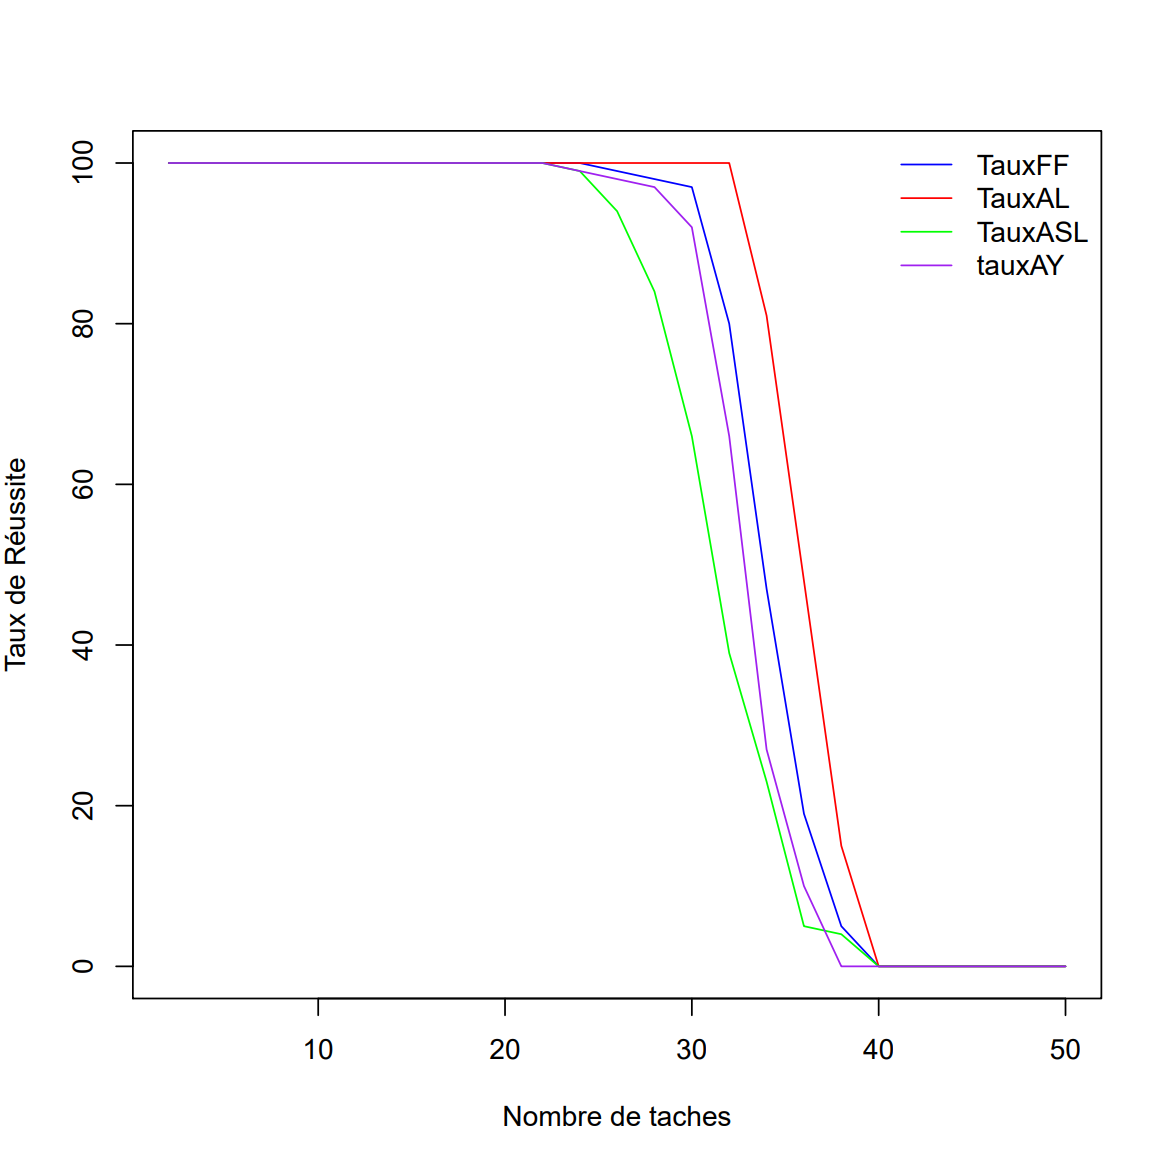
\includegraphics[scale = 0.35]{images/TauxReussite}
    \caption{Taux de reussite sur 100 essais en fonction du nombre de tâches}
\end{figure} 
\begin{figure}[!ht]
    \center
    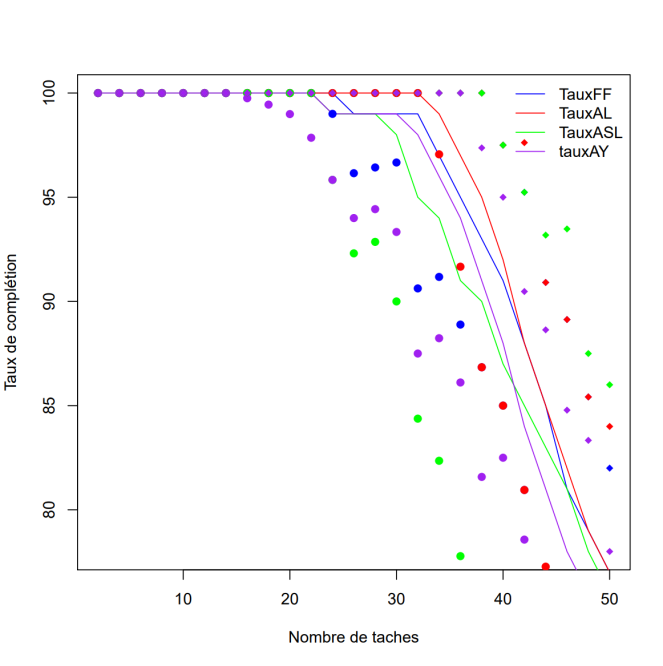
\includegraphics[scale = 0.5]{images/TauxCompletion}
    \caption{Taux de reussite sur 100 essais en fonction du nombre de tâches}
\end{figure}
\begin{figure}[!ht]
    \center
    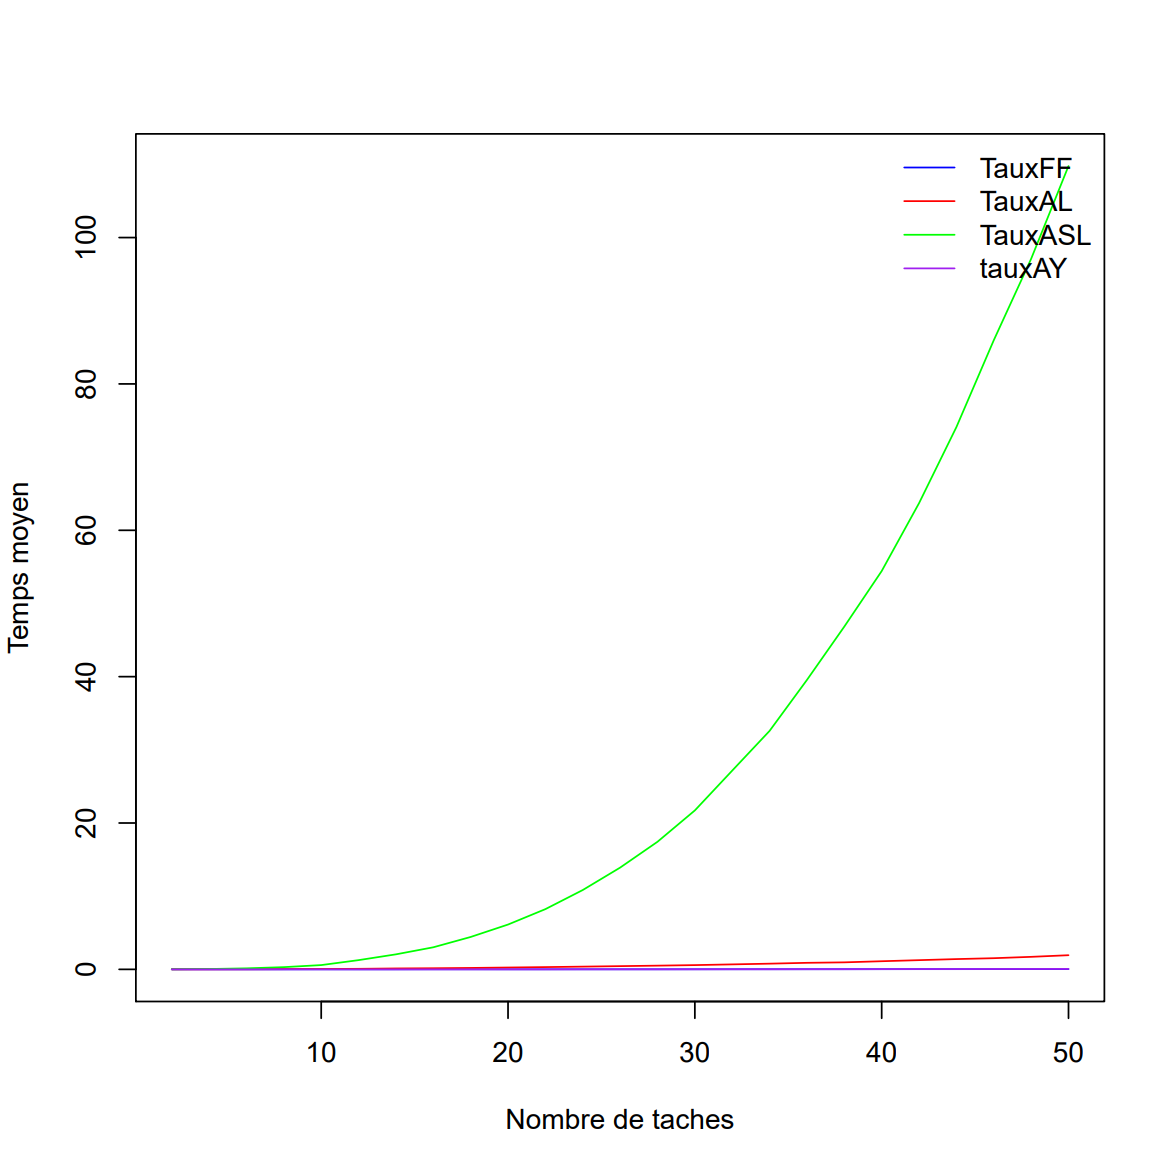
\includegraphics[scale = 0.4]{images/TempsMoyen}
    \caption{Taux de reussite sur 100 essais en fonction du nombre de tâches}
\end{figure}
\end{document}